\documentclass[11pt]{extarticle}


%%%% french character
\usepackage[french]{babel}
\usepackage[T1]{fontenc}
\usepackage[utf8]{inputenc}


%%%% useful package
\usepackage[left=1.8cm, right=1.8cm, top=1.9cm, bottom=2.4cm]{geometry}
\usepackage{subcaption} % for figure caption
\usepackage{graphicx} % image
\usepackage{tabularx} % table
\usepackage{capt-of} % caption for table
\usepackage{longtable} % aligned enumeration
\usepackage{enumitem} % enumeration
\usepackage[table]{xcolor} % color in table
\usepackage{amsmath} % math
\usepackage{amssymb} % math
\usepackage[many]{tcolorbox} % colored box
\usepackage{fancyhdr} % headers
\usepackage[colorlinks=true,linkcolor= Prune,citecolor=black,filecolor=black,urlcolor=Prune]{hyperref} % for link
\usepackage{wrapfig} % to wrap text around figures
% \usepackage{siunitx} % for pretty numbers
\usepackage{gensymb}
\usepackage{chemist}
\usepackage{physics}
\input{insbox}

%%%% package set-up
\usetikzlibrary{calc, positioning} % for coordinate calculation and text alignement
\captionsetup{font=small}


%%%% settings
\setlength{\parskip}{0cm}
\setlength{\parindent}{0.8cm}
\renewcommand{\baselinestretch}{1}


%%%% small macros
\newcommand*{\hham}{\hat{\mathcal{H}}}
\newcommand{\unit}[1]{\; \mathrm {#1}}
\newcommand{\ex}{\mathrm {e}}
%\newcommand{\deriv}{\mathrm {d}}
\newcommand{\boltz}{k_{\mathrm{B}}}
\newcommand{\timeD}[1]{\frac{\deriv #1}{\deriv t}}
\newcommand{\partialD}[2]{\frac{\partial #1}{\partial #2}}
\newcommand{\vect}[1]{\mathbf {\mathcal {#1}}}
\newcommand{\horizontalLine}{\rule{\linewidth}{0.5mm}}
\newcommand{\emptyFrac}{\phantom{\frac{1}{1}}}
\newcommand{\Ihm}{\mathrm{I}_{\mathrm{h}}}
\newcommand{\Ih}{$\mathrm{I}_{\mathrm{h}}\;$}
\newcommand{\Ic}{$\mathrm{I}_{\mathrm{c}}\;$}
\newcommand{\It}{$\mathrm{I}_{\mathrm{t}}\;$}
\newcommand{\Isd}{$\mathrm{I}_{\mathrm{sd}}\;$}
\newcommand{\noSpaceIh}{$\mathrm{I}_{\mathrm{h}}$}
\newcommand{\noSpaceIc}{$\mathrm{I}_{\mathrm{c}}$}
\newcommand{\noSpaceIt}{$\mathrm{I}_{\mathrm{t}}$}
\newcommand{\Nhex}{N_{\mathrm{hex}}}
\newcommand{\Ncub}{N_{\mathrm{cub}}}


\newcommand{\PhDTitle}{\'{E}tude par Résonance Magnétique Nucléaire du magnétisme quantique dans les composés kagomé barlowite et claringbullite substitués au zinc} 

%%%% color
\definecolor{lightgray}{gray}{0.7}
\definecolor{purple}{rgb}{0.58,0,0.82}
\definecolor{darkcyan}{rgb}{0.0, 0.55, 0.50}
\definecolor{darkgreen}{rgb}{0.0, 0.45, 0.20}
\definecolor{Prune}{RGB}{99,0,60} % l14-33 

%%%% bigger macros
%%%% header
% \pagestyle{fancy}
% \lhead { % left header
%   \textbf{\footnotesize \'Ecole normale supérieure}
%   \newline
%   \footnotesize Préparation à l'agrégation de physique-chimie option physique
% }
% \chead{ % central header
% }
% \rhead{ % right header
%   \hfill \textbf{\footnotesize Compte-rendu de leçon de chimie}
%   \newline \hfill
%   \footnotesize 2021-2022
% }
% \renewcommand{\headrulewidth}{0.4pt}


%%%%%%%%%%%%%%%%%%%%%%%%%%%%%%%%%%%%%%%%%%%%%%%%%%%%%%%%%%%%
%%%% blocks for higlight
\newenvironment{highlightBlock}[1]{%
  \begin{tcolorbox}
  [
    breakable, enhanced jigsaw, % to break box over page
    arc = 4mm, % curvature
    title = \textbf{#1}, % title
    coltitle = white, % title font color
    colbacktitle = Prune, % light-gray title
    colback = white, % white background
    colframe = Prune % dark frame
  ]
}
{
  \end{tcolorbox}
}


%%%%%%%%%%%%%%%%%%%%%%%%%%%%%%%%%%%%%%%%%%%%%%%%%%%%%%%%%%%%
%%%% ball of colour with text
\newcommand\ballText[2]{%
  \shorthandoff{;}
  \tikz \node[fill, circle, color=#2,
              inner sep=0pt, text width=20pt,
              font=\footnotesize, align=center]
        {\textbf{\color{white} #1}};
  \shorthandon{;}
}
\newcommand\cyanBallText[1]{\ballText{#1}{Prune}}

%%%% rectangle of colour with text
\newcommand\rectText[3]{%
  \begin{tcolorbox}
  [
    arc = 1mm, % curvature
    colback = #3, % box color
    colframe = #3, % box color,
    width = 48pt,
    height = 18pt,
    %bean arc,
    halign = center,
    valign = center,
    after
  ]
    \textcolor {#2} {\textbf{#1}}
  \end{tcolorbox}
}
\newcommand\cyanRectText[1]{\rectText{#1}{white}{Prune}}

%%%% rectangle of colour
\newcommand\rect[3]{%
  \shorthandoff{;}
  \tikz \node (rect) [draw, fill, color=#1,
              minimum width=#2,
              minimum height=#3] {};
  \shorthandon{;}
}
\newcommand\cyanRect[2]{\rect{Prune}{#1}{#2}}


%%%%%%%%%%%%%%%%%%%%%%%%%%%%%%%%%%%%%%%%%%%%%%%%%%%%%%%%%%%%
%%%% cv entry
\newcommand{\cvEntry}[2]{
  \noindent
  \rect{#1}{80pt}{2pt}
  \textcolor{#1} {
    \textsc {\textbf {#2}}
  }
}
%%%% paragraph
\newcommand{\sectionPara}[2]{
  \vspace{10pt}
  \noindent
  \rect{#1}{50pt}{2pt}
  \textbf {#2}
}


%%%%%%%%%%%%%%%%%%%%%%%%%%%%%%%%%%%%%%%%%%%%%%%%%%%%%%%%%%%%
%%%% For aligned enumeration (cv entry)
\newenvironment{alignedColumn}{%
  \begin{longtable} { l p{0.8\textwidth} }
}
{
  \end{longtable}
}


%%%%%%%%%%%%%%%%%%%%%%%%%%%%%%%%%%%%%%%%%%%%%%%%%%%%%%%%%%%%
%%%% Section
\newcommand{\boxSection}[1]{%
  \refstepcounter{section}
  % number and text
  \cyanRectText{
    \textbf {\large \arabic{section}}
  }
  
  \vspace{-18pt}
  \hspace{-16pt}
  \textbf{\Large \phantom{right} #1}
  
  % subsection counter update
  \setcounter{subsection}{0}
  \addcontentsline{toc}{section}{\protect\numberline{} #1}
}%



%%%%%%%%%%%%%%%%%%%%%%%%%%%%%%%%%%%%%%%%%%%%%%%%%%%%%%%%%%%%
%%%% Background image
%%%% (1,2): position ; 
%%%% 3: width ; 
%%%% 4: image_name ;
%%%% 5: caption ;
\newcommand{\backgroundImage}[5]{% 
  \begin{tikzpicture}[remember picture, overlay] 
    \node[anchor = north west, inner sep = 0pt] (image)
    at ($ (current page.north west) + (#1 mm, -#2 mm) $) {
      \includegraphics[width=#3] {#4}
    };
    \node[text width=#3, align = center, below = of image] {
      #5
    };
  \end{tikzpicture}
}


%%%% document
\begin{document}
\begin{center}
    \textbf {\Large Mise en perspective didactique d’un dossier de recherche} \\
    \vspace{0.2cm}
    \textbf{Brendan Le Pennec} \\
    \vspace{0.2cm}
    Concours externe spécial de l’agrégation de physique-chimie option physique \\
    Session 2023
  \end{center}

  \boxSection{Parcours universitaire et scientifique}


\vspace{20pt}
\cvEntry{Prune}{Parcours académique et professionnel :}

\begin{alignedColumn}
  
  \textbf{2022-2023 :} &
  Préparation à l’agrégation de physique au centre de Montrouge, \textit{ENS, Sorbonne Université, Paris-Saclay}\\
  %
  \textbf{2018-2021 :} & Thèse de physique de l'Université Paris-Saclay, intitulée \og \textbf{\PhDTitle} \fg{}, sous la direction du Pr. F. Bert, soutenue le Jeudi 02 Décembre 2021 au Laboratoire de Physique des Solides (LPS) à Orsay \\
  %
  \textbf{2017-2018 :} &
  Master 2 Concepts Fondamentaux de la Physique (ICFP), Parcours Matière Condensée, \textit{ENS, UPMC, Paris Diderot, Paris-Saclay}. \\
  %
  \textbf{2015-2018 :} & Magistère de physique fondamentale, \textit{Université Paris-Saclay} \\
  %
  \textbf{2013-2015 :} & 
Classes Préparatoires aux Grandes Ecoles - MPSI/MP, \textit{lycée La Pérouse-Kérichen à Brest} \\  %
\end{alignedColumn}


%%%% Stage
\cvEntry{Prune}{Expériences de recherche (hors doctorat) :}

\begin{alignedColumn}

  \textbf{2018 :} & \'{E}tude par RMN du fluor de la barlowite : un nouveau composé kagomé antiferromégnétique, sous la direction du Pr. F. Bert au \textit{LPS, Orsay} (stage de Master 2)\\
  %
  \textbf{2017 :} &
  Croissance cristalline, caractérisation avancée de nouveaux matériaux quantiques, sous la direction du Pr. B. Gaulin à l'\textit{Université de McMaster, Canada} (stage de Master 1)\\
  %
  \textbf{2016 :} &
  \'Etude de la destruction de la supraconductivité dans des films minces de Vanadium, sous la direction du Dr. C. Marrache-Kikuchi au \textit{CSNSM, Orsay} (stage de Licence 3) \\
  % 
\end{alignedColumn}


%%%% Monitorat
\cvEntry{Prune}{Animation, vulgarisation et expériences d'enseignement :}

\begin{alignedColumn}

  \textbf{Mars 2023 :} & Stage facultatif de 3 jours au lycée Condorcet de Montreuil (de la seconde au BTS) \\
  %
  \textbf{2018-2021 :} & Monitorat de Physique (64h/an) à l'Université Paris-Saclay : \begin{itemize}\setlength{\itemsep}{0.05cm}
  \item travaux dirigés de mécanique (L1),
  \item travaux dirigés et travaux pratiques d'optique géométrique (L1),
  \item travaux dirigés de mathématiques pour la physique (L3-magistère).
  \end{itemize} \\
  %
  \textbf{2018-2021 :} & Représentant des non-permanents au conseil du LPS \\
  %
  \textbf{2018-2021 :} &
  Animation du stand "Supraconductivité" pour la Fête de la science au LPS \\
  \textbf{2016 :} & Tutorat de Physique pour des élèves de L1 en difficulté\\
  \textbf{Depuis 2013 :} & Brevet d'Aptitude aux Fonctions d'Animateur (BAFA)
  %
\end{alignedColumn}

\newpage
  
  \boxSection{Formation, expériences et implications personnelles au regard du métier d'enseignant}
\vspace{2mm}

Tout au long de mon parcours académique mais aussi personnel, j'ai confirmé et développé un enthousiasme instinctif pour le partage et la transmission des savoirs scientifiques et de la vie citoyenne. Je développe dans cette partie les liens entre ma formation scientifique, mes expériences professionnelles et personnelles au regard des compétences attendues d'un professeur agrégé de Physique-Chimie.
\subsection{Expériences professionnelles}
Cet enthousiasme prend ses racines dans mes expériences en tant qu'animateur en centre de loisirs et en colonies de vacances. Ces cadres éducatifs non scolaires ont été des lieux et des moments pour, d'une part, écouter et accompagner des enfants et des adolescents dans leur développement personnel, et d'autre part, générer de la curiosité et faire découvrir le monde complexe dans lequel nous vivons. Par exemple, pour introduire le système solaire à des enfants de 6 à 11 ans en centre de loisirs, j'avais créé une semaine thématique lors de laquelle j'ai mené différentes activités manuelles (création d'une fresque du système solaire) et sportives (entrainement d'un astronaute) en essayant d'introduire quelques notions que je connaissais sur le sujet, de manière didactique à travers ces activités. La formation au BAFA\footnote{Brevet d'Aptitude aux Fonctions d'Animateur} et ces premières expériences d'encadrement m'ont appris l'importance de construire un cadre d'activité, d'en donner les règles et les limites à un public jeune, notamment face à des adolescents qui testent régulièrement ces limites. En tant que futur professeur, je ferai par exemple attention à ce que les règles de vie en classe, en particulier en TP de physique et chimie, soient bien établies dès les premières séances de l'année et régulièrement rappelées. %Mes expériences en colonies de vacances m'ont également permises de me rendre compte de l'importance du dialogue et du sens de la coopération au sein d'une équipe d'encadrement. J'ai pu me rendre compte qu'une bonne coordination et une bonne ambiance au sein d'une équipe se reflètent également au sein des groupes que j'ai pu encadrer. 
\\

Mon intérêt particulier pour l'enseignement des sciences et l'accompagnement des élèves dans leur cursus s'est développé au cours de ma formation universitaire. Lors de mes deux premières années au Magistère de Physique Fondamentale d'Orsay, j'ai pu transmettre et consolider des savoirs scientifiques fondamentaux à travers du tutorat d'élèves en difficulté de première année de licence, par petits groupes de deux ou trois élèves. En discutant avec les élèves au cours des séances, je me suis aperçu que la plupart travaillaient en dehors de leurs études, souvent le week-end, ce qui pouvait expliquer en partie leurs difficultés scolaires. Les problématiques ne sont pas les mêmes dans le secondaire (plutôt des problématiques sociales, familiales ou liées à l'adolescence) mais j'ai pu ainsi comprendre l'importance d'être à l'écoute des élèves au cours de l'année et de les suivre individuellement. En complément de ce suivi, j'envisagerai également, dans un futur rôle de professeur principal, des séances de vie de classe où les élèves pourront remonter et partager collectivement leurs difficultés éventuelles sur le déroulement des enseignements et de leur organisation. Ils pourront ainsi soumettre leurs ajustements au conseil de classe de fin de trimestre par l'intermédiaire de leurs délégués.\\

Motivé par cette première expérience d'enseignement, j'ai eu la chance de pouvoir l'enrichir pendant mon doctorat par un monitorat de trois ans à la faculté des sciences de l'université Paris-Saclay. Cette expérience a confirmé ma vocation de professeur. J'y ai pu appréhender la gestion d'une classe ainsi que la gestion du temps d'une séance et d'un planning de suivi de séances, celui-ci étant contraint par l'avancement du programme et la perspective des examens. J'ai trouvé particulièrement intéressant les séances de TP par demi-groupes et en binômes qui permettaient aux étudiants de se poser entre eux des questions conceptuelles (\og finalement, elle est réelle ou virtuelle l'image à travers un miroir ? \fg) et pratiques dans un temps imparti avec une contrainte de réalisation d'un compte rendu par binôme qui était évalué. Je trouverai intéressant de mettre ponctuellement en place des TP \og moins cadrés \fg ~dans lesquels je donnerai un objectif à atteindre (par exemple : \og démontrer expérimentalement la loi de Descartes sur la réfraction \fg ~) et je laisserai aux élèves la liberté de concevoir et valider un protocole expérimental à l'aide du matériel que j'aurai préalablement défini. Ce sera une occasion pour eux d'être confrontés à la mise en \oe uvre (accompagnée) d'une démarche scientifique. Cette séance pourra être également associée à une séance de recherche documentaire au CDI en lien avec le/la documentaliste.\\

Mon expérience a été marquée par la période de confinement liée à la pandémie de la COVID qui a montré à quel point l'enseignement en distanciel pouvait poser des difficultés. Certains élèves m'avaient fait part de leur détresse liée aux différents confinements. Me rendre disponible et à l'écoute a pu les rassurer en partie et m'a permis de faire remonter l'information auprès des responsables de la licence. J'ai pu ainsi orienter ces étudiants vers le personnel de l'université qualifié pour les prendre en charge. Je continuerai à garder cette attitude dans mon futur métier de professeur. Cette expérience m'a également appris à adapter mon enseignement en utilisant des nouveaux outils informatiques : plateforme de visioconférence, utilisation de tableau blanc interactif pour assurer les TD. Au cours de cette période, j'ai aussi pu découvrir des méthodes d'enseignement innovantes à travers les conférences et expériences confinées du chercheur et vulgarisateur Julien Bobroff \footnote{\url{https://www.youtube.com/results?search_query=julien+bobroff+conférence+confinée}}. Certains pourraient me servir de supports didactiques pour des futures expériences à destination des élèves.\\

En plus de la transmission des savoirs fondamentaux en TD ou en TP, j'ai eu la possibilité d'encadrer des stages de recherche à différents niveaux et sur des périodes plus ou moins longues. De façon évidente, je n'ai pas présenté mon activité de recherche ni abordé les sujets de la même façon suivant l'âge et le niveau des étudiants. Par exemple, pour présenter mon activité de recherche à des élèves de troisième lors du stage de découverte dans un milieu professionnel, j'ai choisi de leur montrer quelques expériences visuelles sur les supraconducteurs (voir la figure \ref{fig:SC}) ou de leur montrer l'imposant liquéfacteur d'hélium présent au laboratoire qui permettait d'appréhender notre thématique de recherche et notre travail expérimental quotidien. J'ai également apprécié co-encadrer trois étudiants (un en licence 3, un en master 1 et une en master 2) lors de leur stage de recherche de fin d'année. La difficulté principale résidait en la définition d'un projet expérimental réalisable dans un temps court (de 6 semaines en licence à 3 mois en master) vis-à-vis des durées de campagnes expérimentales (plusieurs mois en général pour des expériences de RMN, voir la partie 3.2 de ce dossier). %Nous faisions des réunions hebdomadaires informelles de façon à préciser l'orientation du projet en fonction de l'avancement de l'étudiant, de la difficulté et de la longueur des mesures. Cette réflexion se menait en étroite collaboration avec les membres de l'équipe, en particulier avec mes encadrants de thèse. Quotidiennement, la nature des travaux que nous fournissions pouvait être . 
Des travaux de nature bibliographique, expérimentale ou de travail de synthèse pouvaient être réalisés en autonomie afin d'impliquer et responsabiliser au mieux ces étudiants dans leur projet. Pour un de ces étudiants, il a été très difficile de le laisser autonome sur son projet et j'ai dû compenser moi-même un manque de travail. Avec le recul sur cette expérience, j'aurais adapté différemment son stage en lui demandant des synthèses écrites sur le déroulé de son travail et de sa compréhension vis-à-vis de celui-ci par exemple. Ces premières expériences de suivi de projets me semblent être formatrices et me seront utiles pour appréhender la préparation et l'évaluation du grand oral du baccalauréat ou dans le suivi des projets de TIPE de CPGE par exemple.

%J'ai également participé à l'animation d'un stand sur la supraconductivité à destination du grand public dans le cadre de la Fête de la Science à l'UPSaclay. Cette expérience m'a entrainé à adapter mon discours face à un public non nécessairement scientifique.
\subsection{Représentant des non-permanents}
Au-delà de ma propre thématique de recherche, j'ai bénéficié d'un environnement scientifique très riche au sein du Laboratoire de Physique des Solides (LPS) d'Orsay. En prenant le rôle d'un des trois représentants des non-permanents de mon laboratoire, j'ai souhaité porter et participer à des projets de rassemblements et d'animations scientifiques que je trouvais très complémentaire à mon travail de thèse. J'ai organisé par exemple la "journée des non-permanents" de mon laboratoire qui permettait de valoriser les travaux de recherche d'une trentaine de doctorants et post-doctorants de tous les domaines de la physique représentés au laboratoire.\\

Suite aux différentes périodes de confinement, la direction du laboratoire nous a permis de créer et réaliser un séminaire scientifique "Oxy'jeunes" à destination des doctorants et post-doctorants du LPS et du LPTMS, un laboratoire voisin. Ce séminaire avait pour but de développer les échanges scientifiques pluridisciplinaires dans un cadre naturel agréable (l'école de Physique des Houches dans les Alpes) après de longs mois de confinements préjudiciables aussi à la qualité des échanges scientifiques. J'ai pu coordonner l'organisation de ce séminaire, gérer le budget associé à ce projet et réaliser un bilan que j'ai présenté lors du conseil de laboratoire. \`{A} travers mon rôle de représentant des non-permanents, j'ai développé des compétences transverses qui me seront très utiles par exemple dans la participation à la vie d'une équipe pédagogique ou dans l'organisation de voyages scolaires thématiques qui peuvent être des rôles endossés par un professeur agrégé. \\

Je vais à présent présenter mes travaux de thèse, leur contexte et les principaux résultats obtenus. Je mettrai en perspective quelques applications associées aux concepts physiques que j'ai étudiés et utilisés pendant ma thèse dans des propositions d'activités que je pourrai être amené à mettre en place dans des cours de l'enseignement du secondaire et du supérieur.
\vspace{2mm}
  \vspace{2mm}
  
  \boxSection{Activités de recherche}
\vspace{2mm}
\`{A} l'échelle microscopique, la matière est constituée d'atomes autour desquels circulent des électrons. En particulier, dans les cristaux, les atomes sont arrangés périodiquement aux n\oe uds d'un réseau cristallin. Les propriétés physiques des cristaux (électriques, magnétiques, mécaniques, etc) proviennent des interactions entre les atomes, entre atomes et électrons et entre les électrons eux-mêmes. \`{A} cette échelle, ces interactions sont décrites dans le cadre de la mécanique quantique. Il faut donc résoudre l'équation de Schrödinger contenant toutes les informations (interactions pertinentes, géométrie du réseau, etc) décrivant le système considéré. Mais les solides cristallins sont constitués de quelques $10^{23}$ atomes et au moins autant d'électrons ce qui rend malheureusement impossible la résolution analytique et même numérique de l'équation de Schrödinger de manière simple. Aujourd'hui, \textbf{la physique de la matière condensée} s'emploie à comprendre les propriétés physiques des systèmes denses (solides et liquides) en mêlant à la fois les concepts de physique statistique et de physique quantique.\\
Ma recherche s'est portée sur l'étude expérimentale de deux nouvelles familles de matériaux et de leurs propriétés magnétiques dans le cadre de la réalisation expérimentale d'états quantiques originaux appelés \textbf{Liquides de Spins Quantiques (LSQ)}.
\subsection{Vers la réalisation expérimentale de liquides de spins quantiques}
\subsubsection{Contexte historique et enjeux sociétaux}
\begin{wrapfigure}{r}{0.4\textwidth}
    \centering
      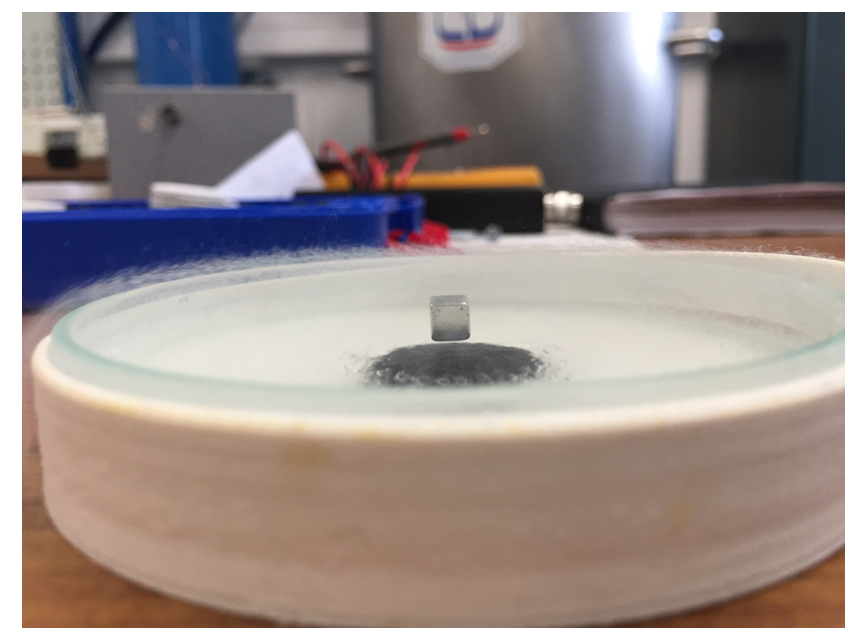
\includegraphics[width=0.4\textwidth]{Fig1.png} 
      \caption{Lévitation magnétique (effet Meissner) du cuprate \chemform{YBa_2Cu_3O_{7+\delta}}. Photo réalisée dans le cadre d'une présentation de la supraconductivité à des élèves de collège. 
      }
      \label{fig:SC}
  \end{wrapfigure}
En 1908, le physicien néerlandais Kamerlingh Onnes découvre la supraconductivité dans le mercure et ses propriétés fascinantes : en dessous d'une certaine température, appelée \og température critique \fg , la résistivité du mercure devient nulle. Autrement dit l'état supraconducteur permet de façon remarquable de transporter du courant sans dissipation par effet Joule. Par ailleurs, si on lui approche un aimant, il se créé des courants de surfaces créant un champ s'opposant à celui qu'on lui impose : c'est l'effet Meissner ou \og lévitation magnétique \fg ~(voir Figure \ref{fig:SC}). La première propriété permet aujourd'hui, par exemple, de générer des champs magnétiques importants et ainsi réaliser les IRM dans les hôpitaux ou encore, de confiner le plasma très chaud dans les projets de fusion nucléaire par confinement magnétique. La seconde propriété permet d'envisager aujourd'hui des trains à lévitation magnétique comme le projet SCMaglev au Japon.\\

Ces propriétés ont été bien comprises dans le cadre de la théorie BCS (Bardeen-Cooper-Schriffer) qui a valu à ses trois fondateurs de partager le prix Nobel en 1956. 
Un des principaux problèmes de l'utilisation des supraconducteurs est le refroidissement des composés car la température critique est de l'ordre de quelques kelvins. Cela pose d'une part des contraintes d'ingénierie importantes et d'autre part cela implique l'utilisation d'hélium liquide qui est un gaz naturel rare (et cher) sur Terre.\\
En 1986, une nouvelle catégorie de supraconducteurs a été découverte : les cuprates. Ces oxydes de cuivre deviennent supraconducteurs pour des températures critiques de l'ordre de $\sim100$~K  ! L'avantage considérable de ces cuprates par rapport aux premiers supraconducteurs est de pouvoir les rendre supraconducteurs avec de l'azote liquide, très facile à produire. Mais, du point de vue de la physique fondamentale, la théorie BCS semble incapable d'expliquer le mécanisme microscopique de la supraconductivité à l'\oe uvre dans ces matériaux. Il s'agit de l'un des grands problèmes de la matière condensée depuis près de 50 ans: quel est donc le mécanisme microscopique à l'origine de la supraconductivité dans les cuprates ? La compréhension de ce mécanisme nous permettrait-elle un jour de réaliser des supraconducteurs à température ambiante ?\\
Plusieurs pistes de réflexion sont aujourd'hui étudiées. L'une d'entre elles repose sur une idée originale du physicien américain P. W. Anderson, prix Nobel en 1977. Il proposa que la \og \textbf{frustration magnétique} \fg ~ associée à des \textbf{interactions antiferromagnétiques} puisse permettre l'apparition de la supraconductivité. Il conceptualisa alors un état que nous appelons aujourd'hui \og \textbf{Liquide de Spins Quantique} \fg (LSQ), et le proposa comme l'état de départ à partir duquel, en le dopant en charges ou en trous, on pourrait obtenir un état supraconducteur.\\
Je vais expliciter les concepts de frustration magnétique et de LSQ ce qui me conduira à présenter les matériaux que j'ai étudiés.


%\begin{highlightBlock}{\textbf{Proposition d'activité 1 :} \'{E}tallonnage d'un capteur de température (Seconde Générale et technologique)}{Dans la thèmatique 3 "Signaux et capteurs" du contenu disciplinaire enseigné en classe de seconde, les  }

\subsubsection{\`{A} la recherche des LSQ sur le réseau kagomé}
\label{Frustration}
Dans un réseau cristallin, les électrons possèdent deux propriétés essentielles. D'une part ils peuvent se déplacer d'un site $i$ à un site $j\neq i$ du réseau cristallin traduisant leur libre propagation dans le réseau. D'autre part ils sont chargés négativement avec une charge électrique élémentaire $q_{e^-}=-e$ ce qui implique une interaction répulsive coulombienne entre les électrons. Il y a donc une compétition entre l'énergie cinétique et l'énergie potentielle électrique au sein de la matière. Lorsque l'interaction coulombienne est importante, on dit que les électrons sont \textbf{fortement corrélés}.\\ %Cette compétition amène une variété importante d'états de la matière. Une façon relativement simple de modéliser mathématiquement cette compétition est l'hamiltonien de Hubbard suivant :
%\begin{equation}
%\hham=-\sum_{i,j,\sigma}t_{i,j}\left(c_{i,\sigma}^{\dagger}c_{j,\sigma}+c_{j,\sigma}^{\dagger}c_{i,\sigma}\right)+U\sum_i n_{i,\uparrow}n_{i,\downarrow}
%\end{equation}
%avec $c_{i,\sigma}^{\dagger}/c_{i,\sigma}$ l'opérateur création/annihilation d'un électron de spin $\sigma=\left\{\uparrow,\downarrow\right\}$ sur le site $i$ et $n_{i,\sigma}=c_{i,\sigma}^{\dagger}c_{i,\sigma}$ le nombre d'électrons de spin $\sigma$ sur le site $i$. Dans cette modélisation, nous avons d'une part négligé les interactions coulombiennes entre électrons de sites cristallins différents et d'autre part, nous avons considéré seulement les électrons d'une seule orbitale électronique (la d pour le cuivre par exemple). Lorsque $U>>t_{i,j}$, le cristal est un isolant électronique dit isolant de Mott car ce sont les interactions entre électrons qui les localisent sur site. 
En plus de leur charge élémentaire, les électrons interagissent à travers une autre de leur propriété intrinsèque : le spin, modélisé par le vecteur $\mathbf{S}$. C'est pourquoi, en 1928, le physicien W. Heisenberg proposa un modèle d'interaction entre les électrons au sein d'un réseau cristallin rassemblant ces énergies cinétique et potentielle en un seul terme d'interaction entre spins électroniques $\mathbf{S}_i$ et $\mathbf{S}_j$. En considérant uniquement des interactions entre spins des électrons premiers voisins (les électrons les plus proches les uns des autres) au sein d'un réseau cristallin, ce modèle s'écrit mathématiquement par l'intermédiaire du hamiltonien de Heisenberg $\hham_H$ :
\begin{equation}
\hham_H = -J\sum_{(i,j)}\mathbf{S}_i\cdot \mathbf{S}_{j}
\end{equation}
avec $J$ l'amplitude de l'interaction appelée communément \textbf{paramètre d'échange}. L'état fondamental magnétique du système correspond à l'état pour lequel cette énergie d'interaction est minimale. Cela nous amène donc à distinguer deux cas suivant le signe de $J$ pour l'état fondamental :
\begin{enumerate}
\item si $J>0$, l'énergie est minimale lorsqu'il y a un alignement des spins entre eux ($\mathbf{S}_i$ et $\mathbf{S}_j$ sont colinéaires et orientés dans le même sens): l'état fondamental du système est alors un état \textbf{ferromagnétique},
\item si $J<0$, l'énergie est minimale lorsqu'il y a un anti-alignement des spins entre eux ($\mathbf{S}_i$ et $\mathbf{S}_j$ sont colinéaires et orientés dans le sens opposé): l'état fondamental du système est alors un état \textbf{antiferromagnétique}.
\end{enumerate}

\begin{figure}[!ht]
\centering
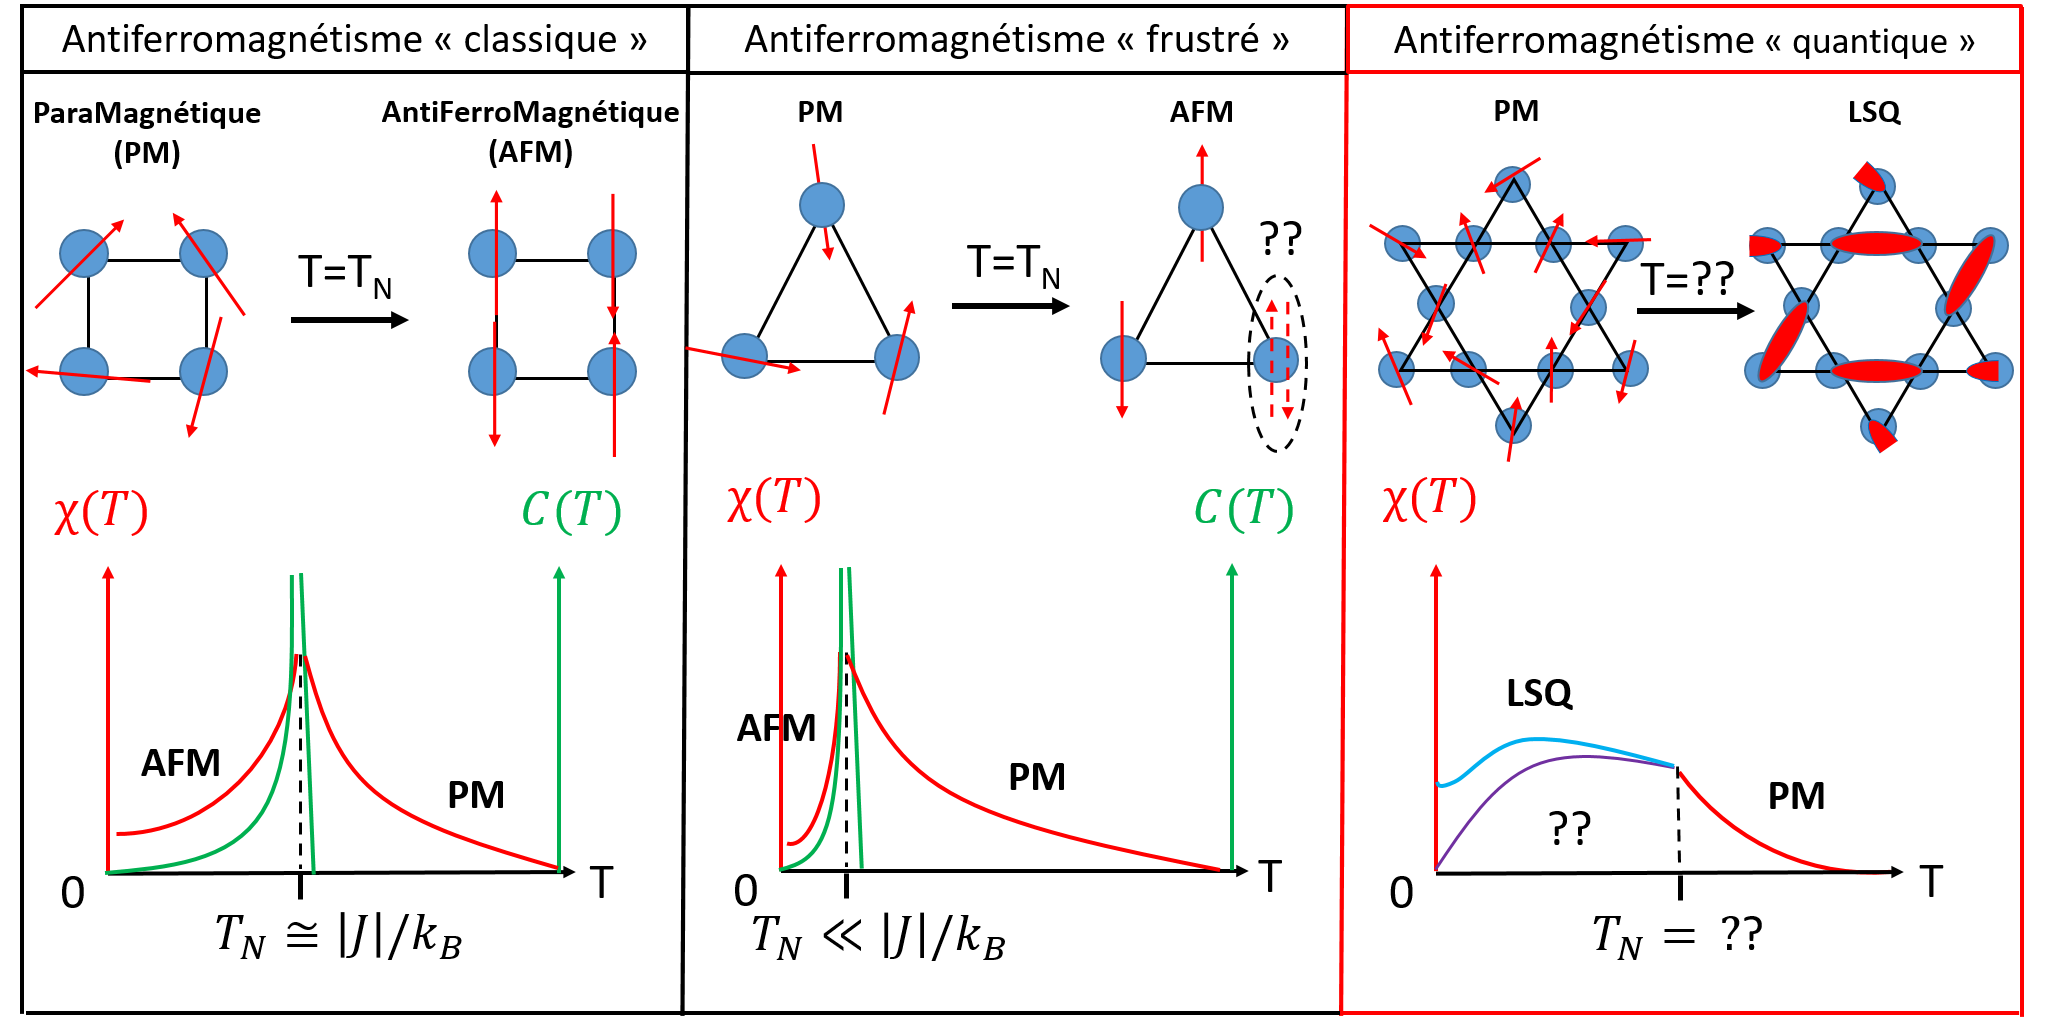
\includegraphics[scale=0.45]{Fig2.png}\caption{\label{fig:magnetisme}Différents cas du magnétisme dans les matériaux antiferromagnétiques avec une interaction proche voisin entre les spins. Les atomes sont représentés par des cercles bleus et les spins électroniques sont représentés par des flèches rouges. Dans le cas du triangle de spins, le spin de droite ne peut pas minimiser en même temps les interactions avec ses deux voisins : il est \og \textbf{frustré} \fg . Dans le cas du réseau kagomé (à gauche), le comportement de la susceptibilité avec la température en dessous de la température de transition (qui est inconnue) est inconnu. Elle peut suivre, par exemple, l'allure théorique de la courbe bleue comme celle de la courbe mauve. Les expériences pourraient trancher entre ces comportements.}
\end{figure}

Nous allons voir par la suite que le cas antiferromagnétique $J<0$ est la condition nécessaire pour avoir un état LSQ. Pour savoir si un matériau est un LSQ, il faut donc déjà reconnaître la présence d'une interaction antiferromagnétique. Cela est possible en étudiant la susceptibilité magnétique ou la capacité thermique $C$ du système en fonction de la température. La susceptibilité magnétique traduit la réponse magnétique du système soumis à un champ magnétique excitateur. Elle est définie par la grandeur $\chi=\frac{M}{H}$, où $M$ est l'aimantation du réseau et $H$ le champ magnétique appliqué.\\
%Dans les oxydes de cuivre, ces interactions sont des interactions dites de \og superéchange \fg passant par des recouvrements des orbitales $p$ de l'oxygène et $d$ du cuivre.\\
Je présente sur la figure \ref{fig:magnetisme} à gauche le cas du réseau carré. Pour des températures $T$ grandes devant $\frac{\abs{J}}{k_B}$, le système est dans un état paramagnétique : les spins sont orientés aléatoirement. En revanche, lorsque $T$ est faible devant $\frac{\abs{J}}{k_B}$, les spins ne peuvent plus s'orienter aléatoirement et s'anti-alignent. La transition entre ces deux états s'effectue à la température $T=T_{N}\sim \frac{\abs{J}}{k_B}$ appelée \textbf{température de Néel}. La signature expérimentale de cette transition est l'apparition d'une divergence à $T=T_{N}$ dans la courbe $C(T)$. En-dessous de cette température, $\chi$ diminue. %Le matériau devient alors antiferromagnétique et sa susceptibilité magnétique diminue (il y a autant de spins qui pointent dans une direction que dans la direction opposée). Cet état est appelé usuellement \textbf{un état de Néel} du nom son inventeur français Louis Néel, prix Nobel de physique en 1970 pour ses travaux sur le magnétisme dans la matière.
Mais que se passe-t-il si la géométrie du réseau est plus complexe ? \\ 
J'ai représenté sur la Figure \ref{fig:magnetisme} au centre l'exemple du triangle de spins. Contrairement au réseau carré, il n'est pas possible de minimiser l'énergie de Heisenberg simplement en anti-alignant les spins entre eux : le système magnétique est dit géométriquement \og \textbf{frustré} \fg. Expérimentalement, la transition magnétique d'un tel système apparaît à des températures bien plus basses que $\frac{\abs{J}}{k_B}$.\\
Allons maintenant un peu plus loin. \`{A} partir de triangles de spins, on peut fabriquer un réseau composé de triangles dont les sommets sont connectés : ce réseau s'appelle le \textbf{réseau kagomé} que j'ai représenté sur la figure \ref{fig:magnetisme} à droite. Dans cette configuration, les théoriciens ont montré que, \textbf{pour des spins $S=1/2$ sur ce réseau, l'état fondamental est un état Liquide de Spins Quantique} : les spins s'associent en paires pour former des états quantiques singulets (d'après les règles de composition de deux moments cinétiques en mécanique quantique, $S_{tot}=1/2+1/2=0$ ou $1$, l'état singulet correspond au moment total $S_{tot}=0$). En revanche, la transition paramagnétique/LSQ se fait continument car il n'y a pas de brisure de symétrie du système. Cela se traduit par l'absence de pic dans la courbe $C(T)$. D'autre part, le comportement précis de la susceptibilité à basse température est actuellement inconnu. Dans la suite, je me focaliserai uniquement sur les mesures de susceptibilité magnétique.
%Pourquoi la dénomination liquide du LSQ ? De la même façon que les corrélations spatiales entre les molécules décroissent très rapidement dans un liquide, les corrélations de spins décroissent très rapidement dans un LSQ.
%On appelle \og \textbf{frustration magnétique} \fg  un système de spins dans lequel il n'est pas possible de minimiser de façon classique les interactions entre spins deux à deux. Nous montrons l'exemple du triangle de spins sur la Figure \ref{fig:magnetisme}.\\
%Il existe théoriquement une multitude d'états LSQ (décroissance lente ou exponentielle des corrélations par exemple) mais il n'existe pas de consensus global dans la communauté scientifique sur lequel est effectivement réalisé pour le réseau kagomé. Il est donc nécessaire de trouver des matériaux modèles cochant tous les critères de la matérialisation d'un LSQ : un réseau kagomé bidimensionnel avec des spins $S=1/2$ et une interaction antiferromagnétique uniquement entre spins premiers voisins.
\subsubsection{De la barlowite ...}
\begin{wrapfigure}{r}{0.4\linewidth}
    \centering
    %\vspace{-15mm}
      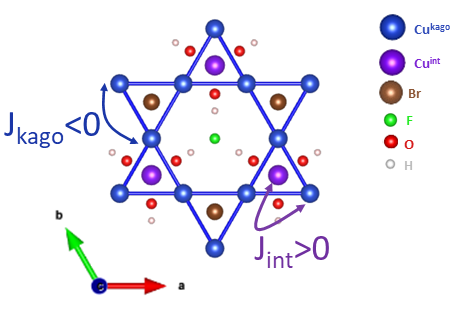
\includegraphics[width=1.\linewidth]{Fig3.png} 
      \caption{
        Structure cristalline de la barlowite obtenue avec le logiciel VESTA.
      }
      \label{fig:barlowite}
  \end{wrapfigure}
Au cours de ma thèse, j'ai étudié expérimentalement deux nouveaux composés présentant des réseaux kagomé et donc possédant potentiellement un état fondamental LSQ : la barlowite \chemform{Cu_{4}(OH)_6FBr} et la claringbullite \chemform{Cu_{4}(OH)_6FCl}. J'ai représenté la structure de la barlowite \chemform{Cu_4(OH)_6FBr} sur la figure \ref{fig:barlowite}. Dans toute la suite de ce dossier, je me focaliserai uniquement sur la barlowite. Nous pouvons voir sur cette figure que, dans la barlowite, des ions cuivres, qu'on appellera Cu$^{kago}$, forment un réseau kagomé parfait dans le plan ($\mathbf{\hat{a}}$,$\mathbf{\hat{b}}$) de la maille hexagonale. Les règles de remplissage de Pauli et Klechkowski pour le cuivre indiquent que le cuivre porte un spin électronique $S=1/2$. De plus, les modèles numériques montrent qu'il existe bien une interaction antiferromagnétique premiers voisins dominante $J_{kago}=-180$~K dans le plan kagomé. En revanche, il existe une autre contribution magnétique importante dans ce matériau. En effet, entre les plans kagomé, il existe des ions cuivres, qu'on appellera Cu$^{int}$ pour cuivres interplans, qui sont couplés ferromagnétiquement aux cuivres des plans kagomé avec une constante de couplage $J_{int}\sim-\frac{J_{kago}}{2}$. Expérimentalement, si on mesure la susceptibilité $\chi$ en fonction de la température dans la barlowite (courbe noire sur la Figure \ref{fig:SQUID}), on observe l'apparition d'une aimantation spontanée, signe d'une transition magnétique vers un état ordonné. \textbf{L'état fondamental de la barlowite n'est donc pas un LSQ}.\\

\begin{highlightBlock}{Activité pédagogique 1 : prise en main d'un logiciel de représentation 3D de mailles cristallines}
\textbf{Contexte :} Dans la thématique \og Une longue histoire de la matière \fg ~enseignée en classe de première générale, la notion de solide cristallin est abordée notamment par la présence de chlorure de sodium naturellement présent dans la mer.\\

\textbf{Objectifs pédagogiques :} \begin{itemize}
 \item Introduire la notion de système cristallin
 \item Prendre en main un logiciel de visualisation
 \item Mesurer un paramètre de maille
\end{itemize}   
\textbf{Déroulement : }L'activité se déroulera en deux séances.
La première commencera par montrer quelques exemples de cristaux sur des diapositives en insistant sur la forme géométrique de ces derniers. J'expliquerai que leurs formes sont dues au fait que la matière s'organise périodiquement à l'échelle microscopique.
Ils pourront appréhender les différentes échelles d'organisation de la matière (roche, cristal, maille, atome).\\
J'introduirai alors la maille cubique à faces centrées dans le cadre d'un modèle de sphères dures en prenant l'exemple du chlorure de sodium (NaCl). Je présenterai les propriétés élémentaires des cristaux : maille élémentaire, paramètres de maille, volume, coordinence, compacité. Les élèves pourront visualiser la maille de NaCl à l'aide d'une fiche de prise en main d'un logiciel libre de représentation des cristaux tel que Avogadro ou VESTA. C'est ce dernier que j'ai largement utilisé en thèse. Une fois la structure visualisée, les élèves pourront mettre en place leurs connaissances sur les cristaux et sur le logiciel de visualisation pour déterminer ses propriétés. \\
Dans la seconde séance, les élèves pourront mesurer expérimentalement la masse volumique d'un système cubique (le fer par exemple) et remonter au paramètre de maille. Ils pourront valider leur résultat en exploitant les outils de mesure des distances entre atomes ou des angles de liaisons chimiques du logiciel de visualisation après obtention de la maille du solide métallique.\\ 
\textbf{Ouverture :} L'activité pourra se conclure par une observation de deux cristallisations de la vanilline réalisées dans des conditions de refroidissement différentes. Je pourrai alors introduire la notion de système amorphe et de conditions de cristallisation faisant un lien avec le programme de SVT sur la dynamique interne de la Terre.
\end{highlightBlock}


\subsubsection{... à la Zn-barlowite.}
\begin{figure}[!bht]
\centering
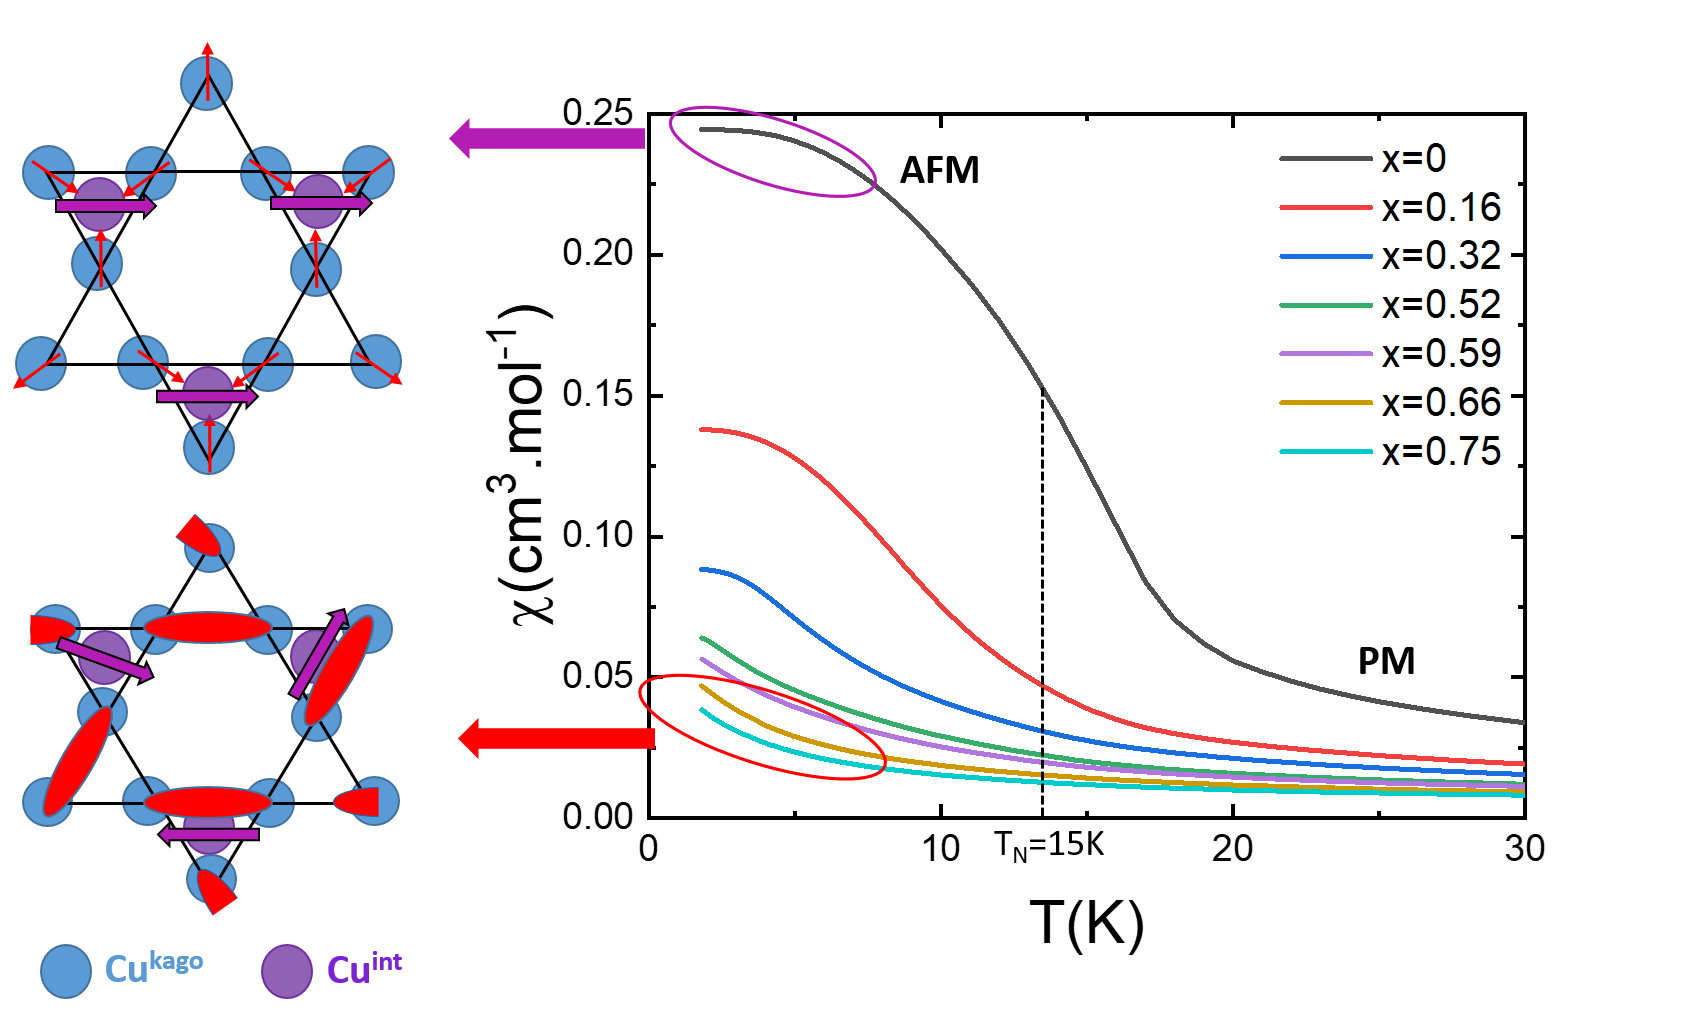
\includegraphics[scale=0.45]{Fig4.png}\caption{\label{fig:SQUID}\'{E}volution de la susceptibilité magnétique mesurée à un champ de 1 tesla en fonction de la température dans la famille des Zn$_x$-barlowites. Pour les faibles valeurs de $x$, l'état fondamental est un état antiferromagnétique, les spins ne s'associent pas en singulets (chaque spin est associé à une flèche sur la figure). Pour $x=0.66$ et $x=0.75$, il y une coexistence entre des singulets (en rouge) sur le réseau kagomé et des spins paramagnétiques sur les cuivres interplans (en violet). La contribution magnétique de ces derniers domine le comportement de $\chi(T)$ à basse température.
}
\end{figure}
Pour faire disparaître ce couplage ferromagnétique et donc espérer stabiliser un état LSQ, l'idée est alors de substituer les cuivres Cu$^{int}$ par des ions non-magnétiques zinc Zn$^{2+}$ pour former les composés Zn$_x$-barlowites de formule chimique Zn$_x$Cu$_{4-x}$(OH)$_6$FBr, où $x$ correspond à la fraction d'ions cuivre substitués par le zinc.\\
J'ai étudié l'évolution des propriétés magnétiques lorsqu'on augmente le taux de substitution en zinc $x$ dans la famille des Zn$_x$-barlowites. J'ai représenté sur la Figure \ref{fig:SQUID} la susceptibilité $\chi$ mesurée à 1 tesla en fonction de la température pour différents échantillons de Zn$_x$-barlowites. Pour des faibles valeurs de $x$, la susceptibilité augmente brutalement à partir de $T_{N}=15$~K sous l'influence du couplage ferromagnétique toujours présent. Les spins ne s'associent pas en singulets comme je l'ai représenté sur la première maille cristalline de cette figure. La somme des vecteurs moments magnétiques de spin est non nulle contrairement à un matériau purement antiferromagnétique, ce qui explique l'augmentation de $\chi$. \\
\`{A} mesure que $x$ augmente, la transition magnétique devient de moins en moins marquée  \textbf{jusqu'à disparaître pour deux échantillons suffisamment substitués ($x=0.66$ et $x=0.75$)}. On peut alors imaginer la coexistence d'un état LSQ sur le réseau kagomé avec des spins qui s'associent en paires et des spins libres sur les cuivres hors plans non substitués comme représenté sur la deuxième maille cristalline de la figure. Toutefois, ces mesures ont été réalisées par un magnétomètre (System of Quantum Interference Device - SQUID) qui est sensible indifféremment à toutes les contributions magnétiques des échantillons. La mesure du magnétisme des plans kagomé reste donc perturbée, en particulier à basse température, par la présence des cuivres interplans résiduels.
%un SQUID mesure la susceptibilité macroscopique $\chi_{tot}(T)$ du système en fonction de la température soit dans le cas d'une Zn$_x$-barlowite partiellement substituée :
%\begin{equation}
%\chi_{tot}(x,T) = (1-x)\chi_{int}(T) + \chi_{kago}(T) + \chi_0
%\end{equation}
%avec $\chi_{int}(T)$ la réponse attribuée aux cuivres hors plans résiduels, $\chi_{kago}(T)$ celle attribuée aux plans kagomé et $\chi_0$ une contribution indépendante de la température. 
Pour pouvoir séparer les différentes contributions magnétiques dans les Zn$_x$-barlowites, j'ai alors utilisé une autre méthode expérimentale particulièrement adaptée pour de telles mesures : la résonance magnétique nucléaire.

\subsection{La Résonance Magnétique Nucléaire (RMN)}
\label{RMN}
La RMN est un outil formidable et puissant pour renseigner sur la nature des liaisons chimiques ou les couplages magnétiques au sein d'un échantillon. Dans les programmes de terminale STL/SPCL ou en chimie de première année de PCSI et BCPST, elle est abordée comme une technique expérimentale permettant de déterminer une structure d'une espèce chimique simple par RMN du proton $^1$H.\\ % Les principaux exercices consistent à déterminer les groupes de protons équivalents, leur multiplicité et leur intégration puis à attribuer les raies observées sur un spectre à ces groupes de protons à l'aide d'une table de déplacements chimiques caractéristiques des liaisons chimiques, comme les liaisons C-H ou O-H par exemple. 
%Je vais montrer qu'en pratique, ses concepts et son utilisation expérimentale regorgent d'exemples illustratifs pour les programmes scientifiques de lycée ou de CPGE.\\
Dans le cadre de ma thèse, j'ai utilisé la RMN comme sonde thermodynamique du magnétisme local des échantillons et espérer s'affranchir ainsi de l'influence des cuivres interplans résiduels.
\subsubsection{Sonder le magnétisme local par RMN}
\begin{figure}[!bht]
\centering
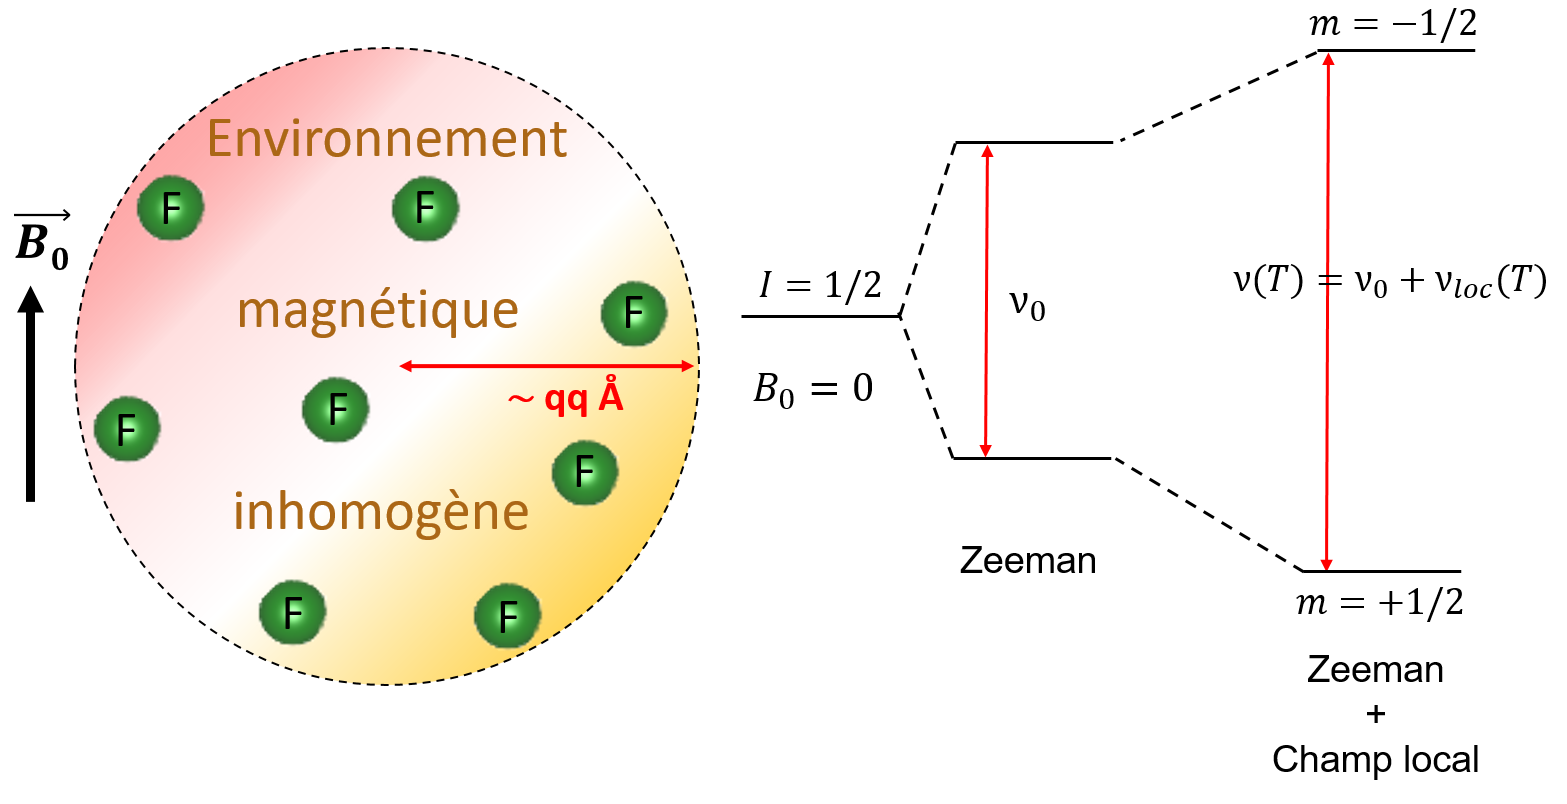
\includegraphics[scale=0.4]{Fig5.png}
\caption{\label{fig:RMN}Principe de la RMN en prenant l'exemple du fluor de spin $I=1/2$ (représenté par les billes vertes).}
\end{figure}

La plupart des noyaux atomiques possèdent un spin nucléaire $\mathbf{I}$. Lorsqu'une population de spins nucléaires est soumise à un champ magnétique extérieur $\mathbf{B}_0$, il y a une levée de dégénérescence en spin des niveaux d'énergie nucléaires : c'est l'\textbf{effet Zeeman}. Prenons pour exemple les noyaux de fluor dans la barlowite qui possèdent un spin $I=1/2$. Comme je l'ai représenté sur la Figure \ref{fig:RMN}, en appliquant un champ magnétique $B_0=\mu_0H$, le niveau d'énergie nucléaire fondamental se scinde en deux sous-niveaux séparés par la fréquence $\nu_{0}=\frac{\gamma_N}{2\pi}B_0$ appelée fréquence de Larmor, avec $\frac{\gamma_N}{2\pi}$ une constante intrinsèque au noyau appelée facteur gyromagnétique. Lorsqu'on soumet cette population de spins à une excitation radiofréquence de fréquence $\nu$, la réponse magnétique de ce système est maximale à la fréquence $\nu=\nu_0$ : c'est la \textbf{résonance magnétique}. %On peut montrer dans le cadre de la mécanique quantique pour un spin $I=1/2$ qu'il se créé des oscillations périodiques de période $1/\nu_{0}$ entre les états $\ket{+\frac{1}{2}}$ et $\ket{-\frac{1}{2}}$ appelées \textbf{oscillations de Rabi}.
\\
Les spins nucléaires sont sensibles à leur environnement magnétique électronique par l'intermédiaire des couplages hyperfins (spins-spins). Cet environnement magnétique décale encore les niveaux d'énergie nucléaires. Ainsi, la fréquence de résonance $\nu_0$ est décalée de $\Delta\nu=\nu(T)-\nu_0$. Ce décalage en fréquence est proportionnel à la susceptibilité locale $\chi_{loc}(T)$ via une constante de couplage appelée constante hyperfine, notée $A_{hf}$. Cette constante nous renseigne sur la force du couplage entre les électrons environnants et le noyau. Nous représentons ce décalage en fréquence par l'intermédiaire de la grandeur $K(T)$ définie comme :
\begin{equation}
K(T) = \frac{\nu(T)-\nu_0}{\nu_0} = A_{hf}\times \chi_{loc}(T) + K_{chem}
\label{equ:shift}
\end{equation}
avec $K_{chem}$ représentant le déplacement chimique qui est indépendant de la température. C'est ce terme qui est référencé en chimie afin de renseigner sur la nature des liaisons chimiques. Le déplacement $K$ est généralement mesuré en $\%$ ou en $ppm$ (partie par million).\\
En mesurant le déplacement des raies RMN et ainsi que leur dynamique en fonction de la température, on accède alors à une mesure du magnétisme local.
\subsubsection{Méthode expérimentale}
Le principe est d'envoyer des trains d'ondes modulés (ou pulses) radiofréquences avec un générateur à travers un circuit passe-bande RLC : c'est \textbf{la RMN impulsionnelle}. La partie cavité radiofréquence peut être une bonne illustration de l'utilisation des filtres RLC résonants abordés en première année de CPGE.\\

\begin{highlightBlock}{Activité pédagogique 2 : étude du circuit RLC série}
\textbf{Contexte : }Au cours du premier semestre de physique, les étudiants de première année de CPGE étudient les signaux physiques sinusoïdaux qui jouent un rôle central dans les systèmes linéaires. Je propose ici une activité consistant à étudier expérimentalement la notion de filtrage par l'exemple d'un filtre passe-bande. C'est ce type de circuit qu'on adapte en permanence pour les mesures de RMN. Cela me permet de donner aux élèves une illustration concrète de l'utilisation de ces circuits électriques classiques.\\
Cette activité introduit des notions des blocs 7 et 8 du programme du premier semestre de MPSI.\\
\textbf{Objectifs : }
\begin{itemize}
 \item Introduire la notion de filtrage 
 \item Réaliser et étudier un filtre passe-bande
 \item Étudier une résonance électrique
\end{itemize}   
\textbf{Déroulement : }L'activité se déroulera en deux séances.\\
La première séance sera constituée d'un cours théorique sur la notion d'impédance complexe et sur l'association en série et en parallèle d'impédances. Les élèves pourront établir et étudier les fonctions de transferts de différents circuits électriques afin de s'approprier les outils mathématiques associés.\\
La deuxième séance sera une séance de TP dans laquelle j'introduirai, à l'aide d'une approche documentaire, le phénomène de résonance en RMN et de son aspect pratique. Les étudiants devront s'approprier ce document et construire une cavité radiofréquence permettant d'isoler un signal fictif RMN à une fréquence $\nu_0$ donnée. Ils devront alors réaliser un filtre passe-bande avec les composants électroniques correctement choisis et devront valider leur démarche par l'étude électrique de leur circuit. Ils pourront tracer le gain en tension en fonction de la fréquence envoyée par le GBF et mesurer la largeur de bande. Ils pourront observer l'effet d'une variation de la résistance sur le facteur de qualité du circuit et sur la largeur de la bande passante. En RMN, la largeur de la bande passante est à comparer à la largeur de raie pour optimiser le temps de mesure. Cette séance sera complétée par l'étude de la résonance en tension aux bornes de la capacité du circuit suivant les valeurs du facteur de qualité.\\
\textbf{Ouverture :} Je pourrai leur donner à étudier en devoir maison l'analogie mécanique d'un circuit RLC série, par exemple un amortisseur de voiture ou un accéléromètre.
%\begin{wrapfigure}{r}{0.4\linewidth}
  %  \centering
 %   \vspace{-5mm}
   %   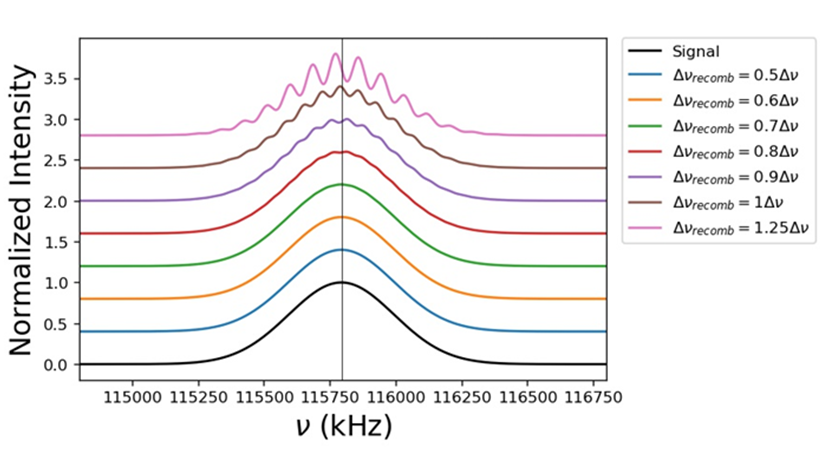
\includegraphics[width=1.\linewidth]{Fig7.png} 
  %    \caption{
   %     Effet d'une recombinaison par un filtre gaussien de largeur $\Delta\nu$. Si le pas de la recombinaison $\Delta\nu_{recomb}$ est trop faible, le spectre RMN est déformé.
     % }
     % \label{fig:Filtre}
  %\end{wrapfigure}
%Cette première séance pourra être complétée par un projet de simulation numérique de l'effet d'une recombinaison spectrale par un filtre gaussien ou lorentzien sous Python. En effet, dans la majorité des cas en RMN, les raies spectrales sont bien plus larges que la largeur du filtre passe-bande radiofréquence. Pour ne manquer aucune partie du spectre, il faut recombiner (\textit{i.e.} sommer avec un certain pas en fréquence) les parties du spectre RMN coupées par la largeur du filtre. Les étudiants seront amenés à manipuler la fonction gaussienne et lorentzienne, leur forme et leur largeur à mi-hauteur.

\end{highlightBlock}
L'échantillon étudié est contenu dans la bobine de ce circuit dont l'axe est orthogonal à $\mathbf{B}_0$. \`{A} l'équilibre, l'aimantation nucléaire de l'échantillon est parallèle à $\mathbf{B}_0$. On envoie alors dans la bobine un pulse radiofréquence d'une certaine largeur temporelle qui bascule l'aimantation nucléaire dans le plan contenant l'axe de la bobine excitatrice. L'aimantation précesse autour de $\mathbf{B}_0$ créant par induction une force électromotrice alternative de quelques $\mu$V dans la bobine. Ce signal est appelé \og décroissance d'induction libre \fg ~ (FID : \textbf{F}ree \textbf{I}nduction \textbf{D}ecay). On l'enregistre ensuite par ordinateur ce qui permet, après transformée de Fourier, de visualiser le spectre RMN. Nous pouvons retenir qu'\textbf{un spectre représente l'histogramme des noyaux résonants à la fréquence $\nu$ et à la température $T$}. Ainsi, le barycentre de la raie représente la valeur moyenne du champ local ressenti par les noyaux et la largeur de raie représente la distribution de ce champ local. La force de la RMN est de pouvoir distinguer \textit{a priori} différentes contributions magnétiques si les noyaux n'ont pas tous le même environnement magnétique (voir figure \ref{RMN}). \\
L'échantillon est placé dans un cryostat qui nous permet d'étudier ses propriétés en fonction de la température (de 300K jusqu'à 1.2K typiquement). Ce cryostat est lui-même placé dans un cryostat plus large contenant une bobine supraconductrice permettant d'atteindre des champs magnétiques $\mathbf{B}_0$ très importants (jusqu'à $14$~T).
%\begin{highlightBlock}{Fonctionnement d'un cryostat (ou vase Dewar ? (CPGE 2ème année)}
%Voir Portelli. Illustration de synthèse du cours de thermodynamique sur les transferts thermiques. Bilan thermique à travers une surface cylindrique. Pour supprimer la conduction thermique : vide entre les parois. Rappel de la loi de Stephan et de ces conditons d'application. Pour minimiser le rayonnement émis par le fluide assimilé à un corps noir : peinture métallique réfléchissante. Utilisation de conducteur thermique adapté. Echelle de température et étalonnage d'un thermomètre à travers l'exemple de la résistance platine ou Cernox ou thermocouple ? Principe du super-isolant ?
%\end{highlightBlock}
Une des difficultés expérimentales en RMN est de maximiser le rapport signal sur bruit pour minimiser le temps d'acquisition d'un spectre. Suivant les temps de relaxation au sein d'un échantillon, de la largeur de raie, de la quantité d'échantillon disponible, du champ appliqué, de la température et de la nature du noyau sonde, certains spectres prennent typiquement plusieurs jours d'acquisition pour une température donnée. Les études RMN que j'ai réalisées ont été des campagnes expérimentales qui ont duré de plusieurs mois à un an pour permettre l'acquisition des mesures.
%\subsubsection{Gap ou pas gap ?}
%La RMN permet de mesurer des énergies de l'ordre de la fréquence de travail $\nu_{0}$ soit de l'ordre de quelques mK (ou 0.5meV) à 100MHz. Autrement dit, c'est une technique spectroscopique très sensible comparée aux excitations typiques (phonons, magnons, etc...) dans la matière. Le grand débat dans la communauté des LSQ est la présence ou l'absence de gap dans le spectre d'excitations des LSQ. Typiquement, les modèles prédisent un gap de l'ordre de $\sim 0.05J_{kago}\sim10$~K, largement mesurable par RMN. Répondre à cette question permet de contraindre fortement l'état fondamental du modèle HAFK et de progresser sur la compréhension des LSQ.\\
%Par la mesure de la susceptibilité locale et la dynamique du champ magnétique local, on prévoit deux types de comportements discriminables par RMN :
%\begin{enumerate}
%\item Si le LSQ est gappé, alors $\chi_{loc}(T)\propto e^{-\frac{\Delta}{T}}$
%\item Si le LSQ n'est pas gappé, alors $\chi_{loc}(T)\propto T^{-\alpha}$ avec $\alpha>0$ une constante.
%\end{enumerate}
\subsection{RMN dans la Zn$_{0.75}$-barlowite}
\label{Résultats}
\subsubsection{Mesure de la susceptibilité locale }
\begin{figure}[!h]
\centering
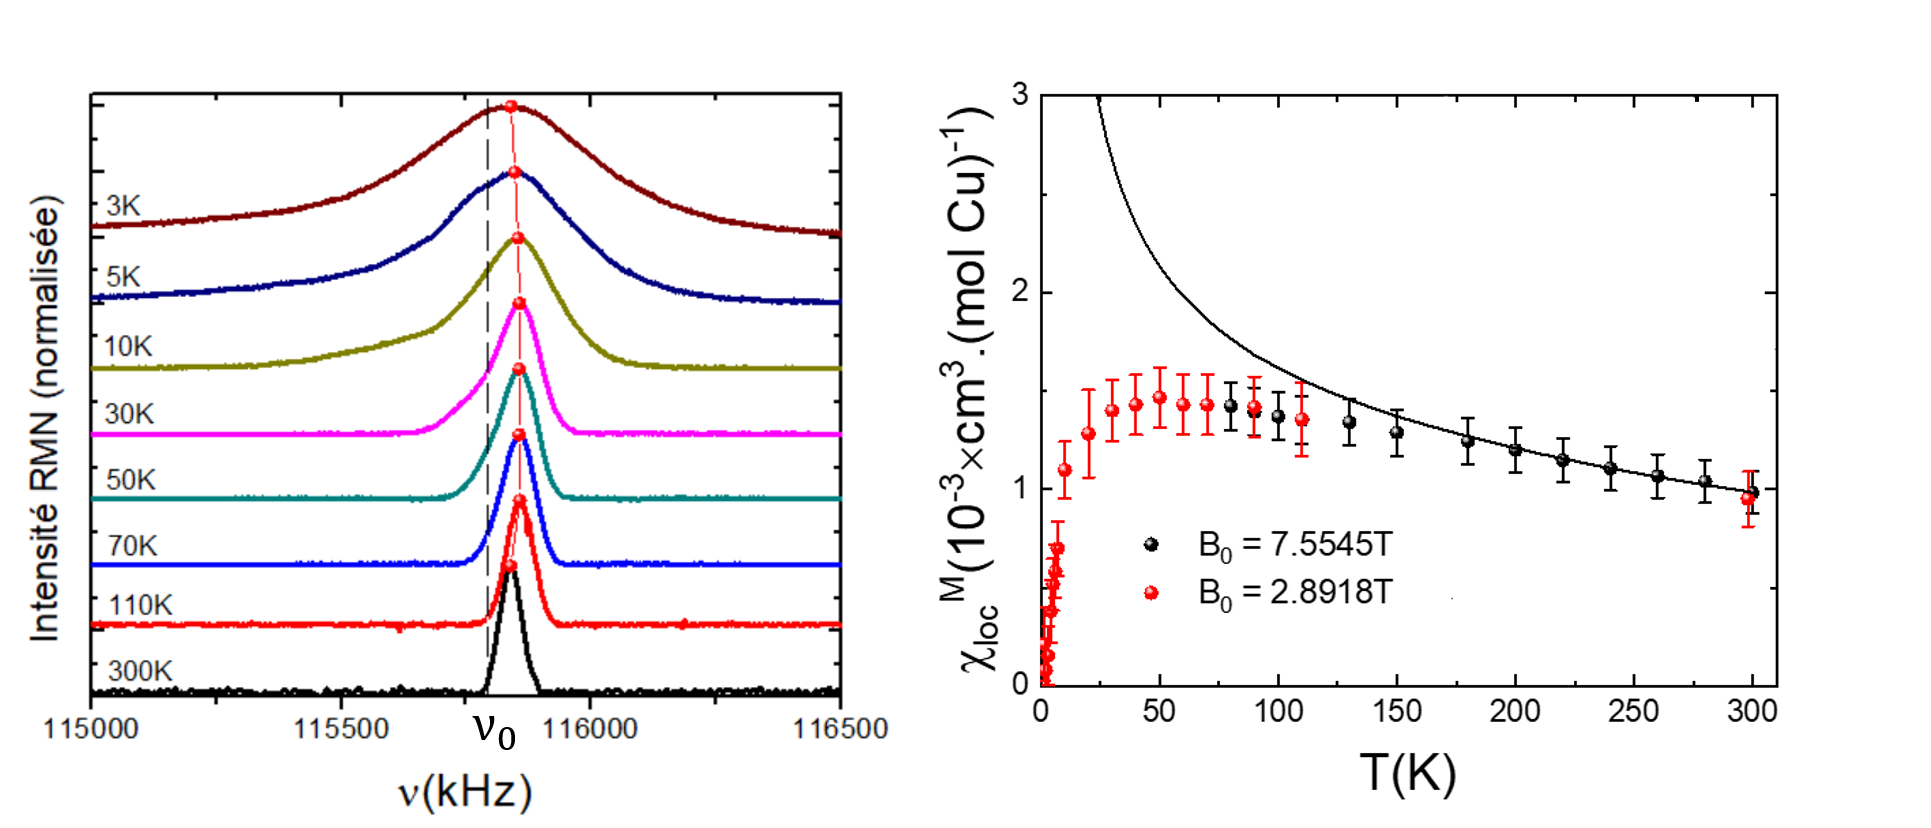
\includegraphics[scale=0.45]{Fig6.png}
\caption{\label{fig:Fluor}\`{A} gauche : spectres RMN du fluor en fonction de la température dans la Zn$_{0.75}$-barlowite mesurés dans un champ $B_0=2.8918$~T. Les points rouges pointent le maximum de la raie. La ligne verticale en pointillées représente la fréquence de référence $\nu_{0}=\frac{\gamma_{Fluor}}{2\pi}B_0=115826$~kHz pour le fluor. \`{A} droite : susceptibilité locale déduite des mesures de gauche en fonction de la température. La ligne continue représente la susceptibilité mesurée par SQUID sur la Figure \ref{fig:SQUID} (ligne couleur cyan  du $x=0.75$).}
\end{figure}
Je présente sur la Figure \ref{fig:Fluor} les spectres RMN du fluor mesurés pour l'échantillon de Zn$_{0.75}$-barlowite à plusieurs températures. On peut voir que la position de la raie RMN, sa largeur, ainsi que sa forme évoluent avec la température. Toute la difficulté consiste à comprendre pourquoi et la réponse n'est pas toujours uniforme.\\
Une première analyse consiste à mesurer la position du maximum de la raie qui correspond au champ moyen ressenti par les noyaux de fluor. J'ai marqué ces maxima par des points rouges sur les spectres de la Figure \ref{fig:Fluor}. On peut voir que ce maximum s'écarte de la fréquence de référence pour $T\in[50,300K]$ puis se rapproche d'elle pour des températures inférieures. \`{A} partir de ce décalage, on peut en déduire la susceptibilité locale $\chi_{loc}$ par l'intermédiaire de l'équation \ref{equ:shift}. Je l'ai représenté sur la figure \ref{fig:Fluor} à droite. Lorsque la température diminue, on peut voir que $\chi_{loc}$ augmente, marque un maximum à $T\sim50$~K puis diminue. Son comportement est complètement différent de la susceptibilité mesurée par SQUID, représentée par la ligne continue sur la figure, puisque celle-ci ne fait qu'augmenter lorsque la température diminue ! \textbf{En l'absence de transition magnétique dans ce matériau, le comportement de $\chi_{loc}$ est bien celui du LSQ présent dans les plans kagomé}.
\subsubsection{Perspectives}
La contribution originale de mon travail repose sur l'analyse comparative des spectres RMN pour différentes valeurs $x$ dans des Zn$_x$-barlowites. J'ai pu montrer qu'il y avait, malgré l'aspect simple de la forme de raie, plusieurs contributions qui se séparent difficilement et qui impactent la position du maximum de la raie. Il y a au moins une contribution provenant du couplage du fluor avec les cuivres interplans résiduels et celle provenant des cuivres du plan kagomé. En particulier, les résultats de la figure 6 de droite proviennent d'une analyse dont les contraintes sont imposées par la forme de raie de quatre échantillons de Zn$_x$-barlowite différents. J'ai montré que l'analyse comparative des différents spectres pour plusieurs valeurs de $x$ est le bon moyen pour identifier la contribution intrinsèque aux plans mais est confrontée à d'importantes difficultés expérimentales (faible déplacement de la raie RMN avec la température, mélange des différentes contributions spectrales,  nécessité d'avoir un échantillon avec un faible taux de défauts).\\

Pour pallier ces difficultés, la piste privilégiée est de réaliser la RMN de l'oxygène $^{17}$O, isotope de l'$^{16}$O. Ce noyau possède un spin nucléaire $I=5/2$ qui a l'avantage d'être bien mieux couplé au magnétisme des plans kagomé. En revanche, du fait de sa très faible quantité naturelle, il faut fabriquer les composés avec de l'eau enrichie à l'$^{17}$O. Les synthèses sont délicates mais les premiers résultats obtenus par RMN de l$^{17}$O sont très prometteurs. Il reste, comme l'étude par RMN du $^{19}$F, à établir une comparaison de différents échantillons enrichis à l'$^{17}$O ou à essayer d'améliorer le taux de substitution en zinc $x$ des échantillons.\\
  \vspace{2mm}
  
  \boxSection{Conclusion générale}
\vspace{2mm}
\`{A} travers mon travail de thèse, j'ai pu mener à bien un projet de recherche à la pointe des questionnements fondamentaux de matière condensée. J'ai étudié l'évolution des propriétés magnétiques de la barlowite lorsqu'on substitue progressivement une partie de ses cuivres interplans par du zinc dans le but de découpler magnétiquement les plans kagomé et espérer réaliser un liquide de spins quantique. Mes travaux ont permis la compréhension des spectres RMN dans ces matériaux et la mise en place d'une méthode fiable pour isoler la contribution intrinsèque des plans kagomé, celle-ci étant sujette à d'importants débats dans la communauté scientifique du magnétisme frustré. \\

Il m'a tenu à c\oe ur d'effectuer une mission d'enseignement à la faculté des sciences d'Orsay en complémentarité de ce travail de recherche. Cette expérience a été déterminante dans mon choix de préparer pendant un an le concours de l'agrégation externe spéciale au centre de préparation de Montrouge. Cette formation m'a permis de réinvestir des connaissances et des compétences apprises en thèse afin de prendre du recul sur la physique et la chimie dans la perspective de mon futur métier de professeur dans ces disciplines.\\

Mon travail de thèse revêt d'une dimension expérimentale importante que j'ai souhaité mettre en valeur dans ce dossier. Devant mes futurs élèves, je souhaiterai d'autant plus insister sur l'aspect expérimental de la physique et de la chimie, qui est parfois nécessaire et cruciale pour, d'une part vérifier ou explorer des modèles théoriques, et d'autre part comparer à d'autres études publiées dans la littérature. Le concept de démarche scientifique illustré par la mise en \oe uvre de protocoles expérimentaux est une méthode que je souhaiterai transmettre à mes futurs élèves.
%
%Le principe du cryostat peut être une belle illustration de l'utilisation des principes de la thermodynamique et de la caractérisation des échanges thermiques pouvant être vues en 2ème année de CPGE.
  
  %\input{monitorat}
\end{document}
